\documentclass[
11pt, % The default document font size, options: 10pt, 11pt, 12pt
%codirector, % Uncomment to add a codirector to the title page
]{charter} 




% El títulos de la memoria, se usa en la carátula y se puede usar el cualquier lugar del documento con el comando \ttitle
\titulo{Moderación automática de facturas y comprobantes de pago} 

% Nombre del posgrado, se usa en la carátula y se puede usar el cualquier lugar del documento con el comando \degreename
%\posgrado{Carrera de Especialización en Sistemas Embebidos} 
%\posgrado{Carrera de Especialización en Internet de las Cosas} 
\posgrado{Carrera de Especialización en Intelegencia Artificial}
%\posgrado{Maestría en Sistemas Embebidos} 
%\posgrado{Maestría en Internet de las cosas}

% Tu nombre, se puede usar el cualquier lugar del documento con el comando \authorname
\autor{Ing. Daniel Calderón Rave} 

% El nombre del director y co-director, se puede usar el cualquier lugar del documento con el comando \supname y \cosupname y \pertesupname y \pertecosupname
\director{Sin Director asignado}
\pertenenciaDirector{-} 
% FIXME:NO IMPLEMENTADO EL CODIRECTOR ni su pertenencia
%\codirector{John Doe} % para que aparezca en la portada se debe descomentar la opción codirector en el documentclass
%\pertenenciaCoDirector{FIUBA}

% Nombre del cliente, quien va a aprobar los resultados del proyecto, se puede usar con el comando \clientename y \empclientename
\cliente{Karenn Márquez}
\empresaCliente{Alquilando}

% Nombre y pertenencia de los jurados, se pueden usar el cualquier lugar del documento con el comando \jurunoname, \jurdosname y \jurtresname y \perteunoname, \pertedosname y \pertetresname.
%\juradoUno{Nombre y Apellido (1)}
%\pertenenciaJurUno{pertenencia (1)} 
%\juradoDos{Nombre y Apellido (2)}
%\pertenenciaJurDos{pertenencia (2)}
%\juradoTres{Nombre y Apellido (3)}
%\pertenenciaJurTres{pertenencia (3)}
 
\fechaINICIO{18 de octubre de 2021}		%Fecha de inicio de la cursada de GdP \fechaInicioName
\fechaFINALPlan{18 de diciembre de 2021} 	%Fecha de final de cursada de GdP
\fechaFINALTrabajo{18 de octubre de 2022}	%Fecha de defensa pública del trabajo final


\begin{document}

\maketitle
\thispagestyle{empty}
\pagebreak


\thispagestyle{empty}
{\setlength{\parskip}{0pt}
\tableofcontents{}
}
\pagebreak


\section*{Registros de cambios}
\label{sec:registro}


\begin{table}[ht]
\label{tab:registro}
\centering
\begin{tabularx}{\linewidth}{@{}|c|X|c|@{}}
\hline
\rowcolor[HTML]{C0C0C0} 
Revisión & \multicolumn{1}{c|}{\cellcolor[HTML]{C0C0C0}Detalles de los cambios realizados} & Fecha      \\ \hline
1.0      & Creación del documento                                 & 18/10/2021 \\ \hline
1.1      & Se completa hasta el punto 5 inclusive                 & 04/11/2021 \\ \hline
%2      & Se completa hasta el punto 7 inclusive
%		  Se puede agregar algo más \newline
%		  En distintas líneas \newline
%		  Así                                                    & dd/mm/aaaa \\ \hline
%3      & Se completa hasta el punto 11 inclusive                & dd/mm/aaaa \\ \hline
%4      & Se completa el plan	                                 & dd/mm/aaaa \\ \hline
\end{tabularx}
\end{table}

\pagebreak



\section*{Acta de constitución del proyecto}
\label{sec:acta}

\begin{flushright}
Buenos Aires, \fechaInicioName
\end{flushright}

\vspace{2cm}

Por medio de la presente se acuerda con el \authorname\hspace{1px} que su Trabajo Final de la \degreename\hspace{1px} se titulará ``\ttitle''. Consistirá esencialmente en la implementación de un sistema para determinar la correspondencia de un recibo de pago con una factura determinada mediante el uso de algortimos de inteligencia artificial, y tendrá un presupuesto preliminar estimado de 600 hs de trabajo y USD 2000, con fecha de inicio \fechaInicioName\hspace{1px} y fecha de presentación pública \fechaFinalName.

Se adjunta a esta acta la planificación inicial.

\vfill

% Esta parte se construye sola con la información que hayan cargado en el preámbulo del documento y no debe modificarla
\begin{table}[ht]
\centering
\begin{tabular}{ccc}
\begin{tabular}[c]{@{}c@{}}Ariel Lutenberg \\ Director posgrado FIUBA\end{tabular} & \hspace{2cm} & \begin{tabular}[c]{@{}c@{}}\clientename \\ \empclientename \end{tabular} \vspace{2.5cm} \\ 
\multicolumn{3}{c}{\begin{tabular}[c]{@{}c@{}} \supname \\ Director del Trabajo Final\end{tabular}} \vspace{2.5cm} \\
%\begin{tabular}[c]{@{}c@{}}\jurunoname \\ Jurado del Trabajo Final\end{tabular}     &  & \begin{tabular}[c]{@{}c@{}}\jurdosname\\ Jurado del Trabajo Final\end{tabular}  \vspace{2.5cm}  \\
%\multicolumn{3}{c}{\begin{tabular}[c]{@{}c@{}} \jurtresname\\ Jurado del Trabajo Final\end{tabular}} \vspace{.5cm}                                                                     
\end{tabular}
\end{table}




\section{1. Descripción técnica-conceptual del proyecto a realizar}
\label{sec:descripcion}
\vspace{5px}
\begin{•}
El proyecto será realizado en la empresa Alquilando, una startup Argentina que presta SaaS (Sotfware as a Service) para el sector inmobiliario en latinoamérica. A través de la plataforma desarrollada por la empresa pueden interactuar inmobiliarias, inquilinos y propietarios de inmuebles, lo que permite onmicanalidad en las comunicaciones y centralización de la gestión de los inmuebles en alquiler que administran las inmobiliarias. Uno de los servicios que presta la plataforma, es permitir que los inquilinos carguen las facturas de los servicios y su correspondiente recibo de pago, luego, ambos documentos deben ser verificados y aceptados por la inmobiliaria, en caso de que la inmobiliaria no pueda comprobar la correspondecia de los dos documentos, deberá rechazar la carga, explicar el motivo y solicitar de nuevo la carga con la información correcta. Los motivos más comunes de rechazo de documentos son, cuando uno de los dos documentos no corresponde con el otro, cuando la información en el recibo de pago no contiene los suficientes datos para comprobar que está relacionado con la factura y, cuando alguno de los dos documentos es ilegible.

Para una inmobiliaria que no es usuaria de la plataforma de Alquilando y que no tiene ningún sistema similar, el proceso de "moderación de facturas y comprobantes de pago" le demanda dedicación exclusiva varios días del mes, esto varía según al volumen de inmuebles que administre la inmobiliaria, este proceso está compuesto por la gestión, moderación y administración de la documentación. A partir de la implementación de la plataforma de Alquilando, la gestión y la administración son considerablemente más eficientes, en cuanto a la moderación, Alquilando la ofrece como un servicio adicional, es así que en lugar de ser la inmobiliaria la que realiza esta tarea, personal de Alquilando lo hace.

Ya sea que la inmobiliaria contrate el servicio adicional o no, esta tarea siempre va a estar a cargo de una persona, pues en Alquilando se cuenta con personal que dedica gran parte de su tiempo a la "moderación de facturas y comprobantes de pago" de inmobiliarias que contrataron este servicio adicional. Por lo tanto, sería de gran utilidad para la empresa encontrar una forma de realizar esta tarea que permita incrementar la eficiencia, al reducir los errores y los costos de tiempo y dinero.

Teniendo en cuenta lo anterior, se encuentra en la tecnología y específicamente en la inteligencia artificial una salida a esta problemática, donde se buscará diseñar un algoritmo que permita verificar automáticamente la correspondencia entre las facturas y los comprobantes de pago cargados por los usuarios de la plataforma, luego enviará un mensaje de confirmación o rechazo (Indicando el motivo) y finalmente actualizará el estado del pago del servicio. Este proceso pretende reducir la intervención del agente inmobiliario y del personal de soporte en un 85\%. Solo se requerirá la intervención humana para aquellos casos en los cuales la información es ilegible o el usuario ha intentado cargar el comprobante más de tres veces y siempre le fue rechazado por el sistema.

La elaboración de un proyecto de estas características, impacta directamente en la propuesta de valor ofrecida por la compañía e incrementa la percepción de valor, no solo por parte de los usuarios de la plataforma sino también de los inversores actuales y potenciales. Actualmente, la empresa cuenta con varios proyectos de mejora enfocados en la experiencia del usuario y en establecer una ventaja competitiva en el mercado. Sin embargo, ninguno de ellos está basado en inteligencia artificial, así que poder obtener conocimientos en éste área por parte de la empresa, también busca ser el comienzo de una serie de procesos y servicios que potencialmente puedan basarse en esta tecnología.

A continuación se observa el modelo canvas del proyecto:


\begin{figure}[htpb]
\centering 
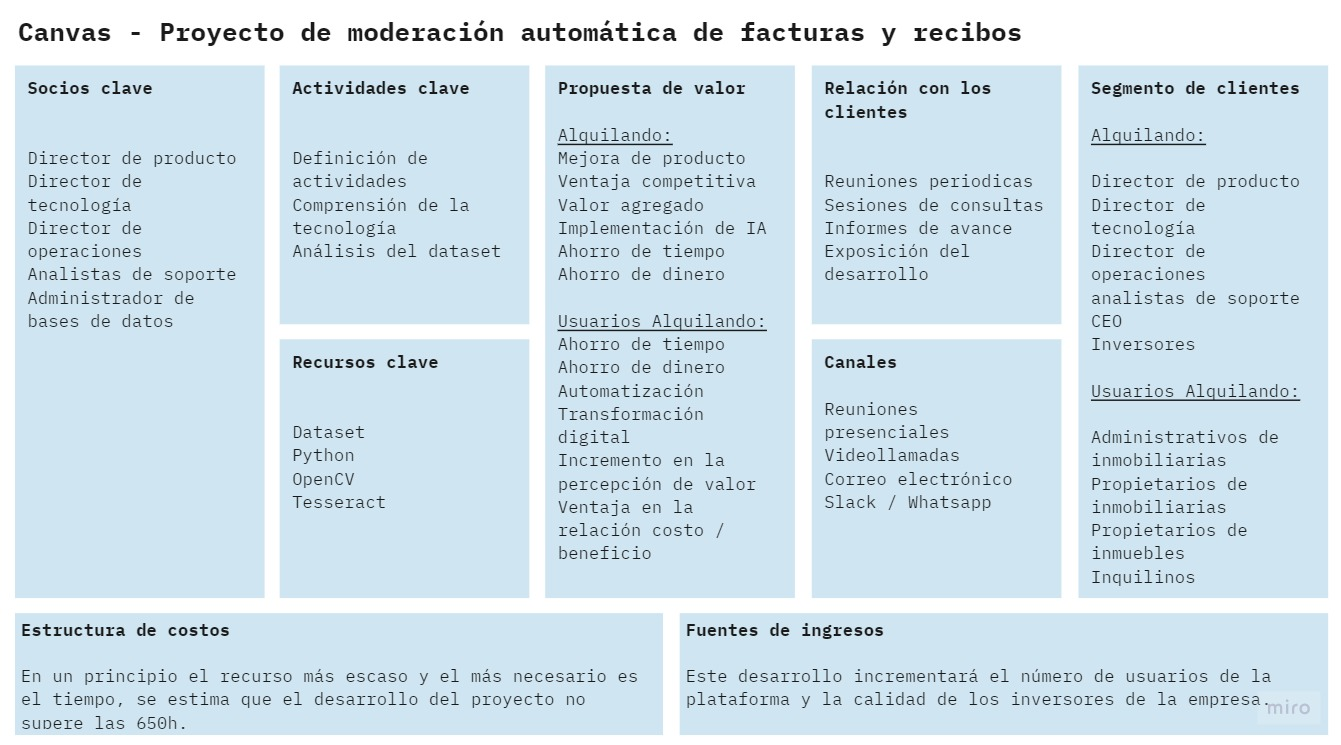
\includegraphics[width=1\textwidth]{./Figuras/Canvas_1.jpg}
\caption{Canvas del proyecto.}
\label{fig:Canvas_1}
\end{figure}

En el modelo canvas, se puede observar que la estructura de costos está enmarcada principalmente por el tiempo a invertir, luego las actividades y recursos clave comprenden básicamente el aspecto tecnológico, al mismo tiempo la propuesta de valor y el segmento de clientes muestran que el impacto que representa este proyecto para la empresa es mucho mayor que el costo de su implementación. 

El desarrollo del proyecto estará basado en la tecnología OCR (Optical Character Recognition) a través de Tesseract, OpenCV y Python. La tecnología OCR se encuentra enmarcada en la tecnología IDP (Intelligent Document Processing) la cual se centra en la automatización de extracción de datos de documentos complejos, bien sea semiestructurados (Facturas, recibos, ordenes de compra, etc.) o no estructurados (Contratos, artículos, cartas, etc.) para transformarlos en  datos estructurados útiles. La tecnología IDP se basa en AI (Artificial Intelligence), ML (Machine Learning), CP (Computer Vision), ICR (Intelligent Character Recognition) y en la ya mencionada OCR para llevar adelante la extracción de información de los diferentes documentos de forma rápida, confiable y precisa.

En la siguiente figura se visualiza un diagrama de bloques del proceso: \newpage

\begin{figure}[htpb]
\centering 
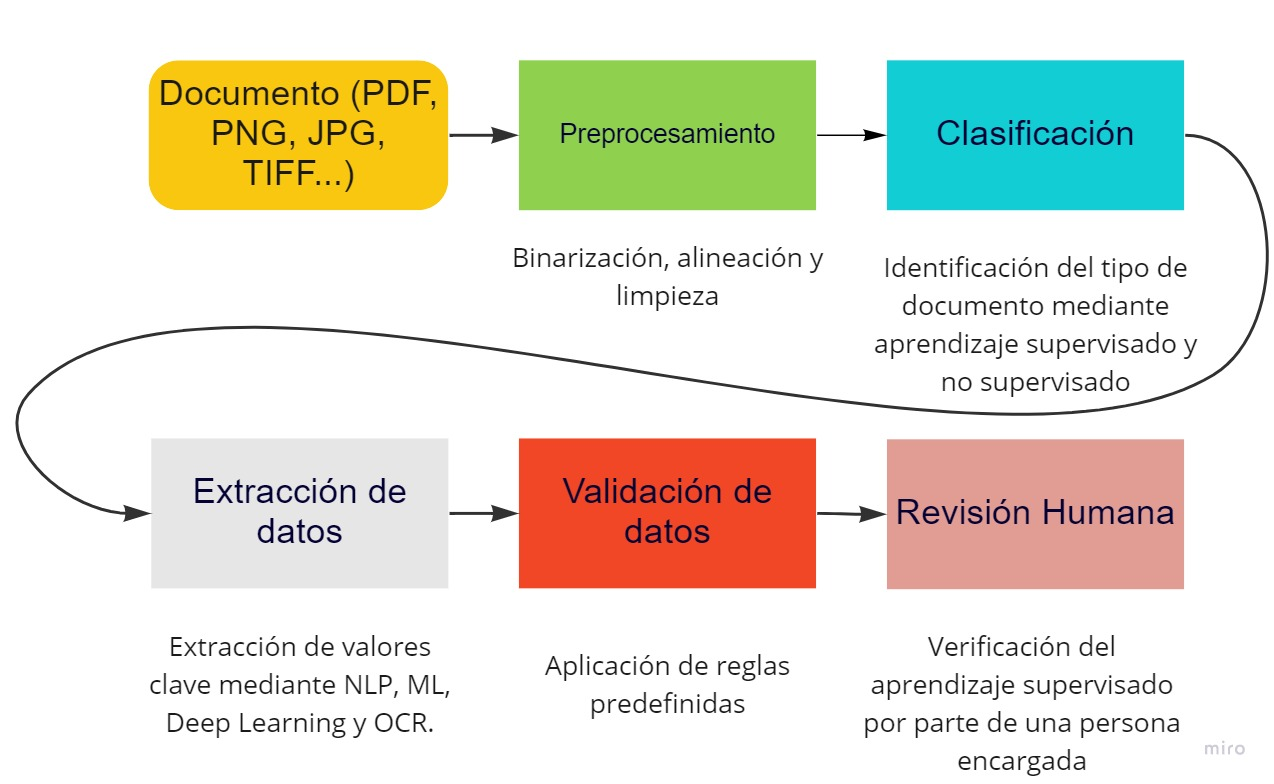
\includegraphics[width=.8\textwidth]{./Figuras/DiagBloq.jpg}
\caption{Diagrama de bloques del proceso.}
\label{fig:DiagBloq}
\end{figure}


Es así como a través de NLP (Natural Language Processing) es posible lograr que el algoritmo pueda reconocer caracteres, símbolos, letras, tablas y todo tipo de características que conformen el documento y sean relevantes para extraer la información de forma estructurada. Este proceso puede ser resumido en las siguientes etapas:

\begin{itemize}
\item Preprocesamiento: se prepara el documento para que su información sea lo más legible posible y de esta forma el algoritmo pueda identificar las diferentes partes del documento y clasificar la información. En esta etapa se realizan tres tareas:
\begin{enumerate}
\item Binarización: se modifica el color del documento reduciéndolo a blanco y negro (0 y 1).
\item Alineación: se ubica el documento en una posición que facilite su lectura.
\item Limpieza: se retiran todos aquellos detalles que pueden ser confundidos por caracteres por el algoritmo.
\end{enumerate}

\item OCR: consiste en identificar los diferentes caracteres que conforman el documento para su extracción. Este proceso se realiza con alguna de las diferentes técnica de visión por computadora que pueden ser:

\begin{enumerate}
\item Utilizar filtros para separar los caracteres del fondo.
\item Aplicar la detección de contornos para reconocer los caracteres filtrados.
\item Utilizar la clasificación de imágenes para identificar los caracteres.
\end{enumerate}

\item Extracción de la información: una vez identificados todos los caracteres que componen el documento es necesario determinar cuál es la información que debe ser extraída. Para esto existen métodos como:

\begin{itemize}

\item Extracción basada en reglas: en este caso el modelo identifica una serie de caracteres que componen una palabra buscada y determina que la línea siguiente está relacionada, por ejemplo, los caracteres que siguen a “Periodo de facturación” corresponden a este dato.
\item Extracción basada en aprendizaje: a través de machine learning y deep learning se entrena al algoritmo con un conjunto de datos que conforme crece aumenta la precisión del modelo.
\end{itemize}

\item Registro de información: finalmente, y luego de contar con la información de interés, es necesario definir el formato en el cual será almacenada. Actualmente, el formato JSON es uno de los más usados dado que tiene facilidad de ser convertido a otros formatos.
\end{itemize}


%\vspace{25px}

%El tamaño de la tipografía en TODAS las figuras debe ser adecuado para que NO pase lo que ocurre acá, donde el lector debe esforzarse para poder leer el texto. Los colores usados en el diagrama deben ser adecuados, tal que ayuden a comprender mejor el diagrama, preferentemente en la gama de colores pastel.


\end{•}


\section{2. Identificación y análisis de los interesados}
\label{sec:interesados}

\begin{•}%{red} 
%Nota: (borrar esto y todas las consignas en color rojo antes de entregar este documento).
 
%Es inusual que una misma persona esté en más de un rol, incluso en proyectos chicos.
 
%Si se considera que una persona cumple dos o más roles, entonces sólo dejarla en el rol más importante. Por ejemplo:

%\begin{itemize}
%\item Si una persona es Cliente pero también colabora u orienta, dejarla solo como Cliente.
%\item Si una persona es el Responsable, no debe ser colocado también como Miembro del equipo.
%\end{itemize}

%Pero en cambio sí es usual que el Cliente y el Auspiciante sean el mismo, por ejemplo.

\begin{table}[ht]
%\caption{Identificación de los interesados}
%\label{tab:interesados}
\begin{tabularx}{\linewidth}{@{}|l|X|X|l|@{}}
\hline
\rowcolor[HTML]{C0C0C0} 
Rol           & Nombre y Apellido & Organización 	& Puesto 	\\ \hline
Auspiciante   &  -                & -             	& -     	\\ \hline
Cliente       & \clientename      &\empclientename	& Administradora de producto   	\\ \hline
Impulsor      &     -             &              -	&        -	\\ \hline
Responsable   & \authorname       & FIUBA        	& Alumno 	\\ \hline
Colaboradores &  Javier La Banca  & Alquilando      & Director de tecnología 	\\ \hline
			  & Ariel Rodeiro     & Alquilando      & Director de operaciones \\ \hline
Orientador    & \supname	      & \pertesupname 	& Director Trabajo final \\ \hline
Equipo        & \authorname       & \empclientename & Consultor de Procesos\\ \hline
Opositores    &     -             &          -      &    -    	\\ \hline
Usuario final &  Equipo de soporte al cliente       &   Alquilando         & - \\ \hline
			  & Equipo administrativo de inmobiliarias & Aquilando & Usuario \\ \hline
\end{tabularx}
\end{table}

Descripción de roles dentro del proyecto:

\begin{itemize}

\item Cliente: será \clientename, que en su posición como administradora de producto (product manager) fue quien a partir de la posibilidad de desarrollar un proyecto basado en inteligencia artificial, encontró que aplicar esta tecnología en el proceso de moderación de comprobantes de facturas y recibos de pago sería una mejora considerable para el producto, los procesos internos y la experiencia de los usuarios.
\item Colaboradores: Javier La Banca, como cofundador de la empresa y director de tecnología proveerá el set de datos necesario para llevar adelante el proyecto.
\item Equipo: en un principio el equipo estará conformado por el \authorname, quién llevará adelante el proyecto, conforme se avance en el desarollo del mismo se determinará la necesidad de incluir más participantes al equipo.
\item Usuario final: estos serán principalmente dos, el equipo de soporte al cliente de la empresa, quienes actualmente son los encargados de realizar la tarea manual que se pretende realizar a través de inteligencia artificial, y luego, los administradores de las inmobiliarias clientes de Alquilando. Para ambos, la finalización con éxito de este proyecto representa un considerable ahorro de tiempo que podrán destinar a otras tareas que les pemitan agregar valor a su actividad.
\end{itemize}



\section{3. Propósito del proyecto}
\label{sec:proposito}

\begin{•}%{red}
%¿Por qué se hace el proyecto? ¿Qué se quiere lograr? 

%Se recomienda que sea solo un párrafo que empiece diciendo ``El propósito de este proyecto es...''.
El propósito del proyecto es, que mediante Inteligencia artificial se mejore el producto ofrecido por la empresa Alquilando, implementando un algoritmo que permita automatizar la moderación de facturas con sus respectivos comprobantes de pago, y reducir en un 85\% la intervención humana en este proceso, la cual actualmente es del 100\%. 


\end{•}

\section{4. Alcance del proyecto}
\label{sec:alcance}

\begin{•}%{red}
%¿Qué se incluye y que no se incluye en este proyecto?

%Se refiere al trabajo a hacer para entregar el producto o resultado especificado. 

%Explicitar todo lo quede comprendido dentro del alcance del proyecto.

%Explicitar además todo lo que no quede incluido (``El presente proyecto no incluye...'')

Desarrollar un algoritmo basado en la tecnología OCR (Optical Character Recognition) que permita:
\begin{itemize}
\item Procesar documentos e imágenes en formatos tales como pdf, jpg, png, tiff.
\item Realizar un preprocesamiento de la imagen, reduciendo sus colores a blanco y negro, corrigiendo la orientación y eliminando "ruidos".
\item Indentificar el tipo de documento y reconocer los caracteres que lo componen.
\item Aplicar reglas predefinidas que permitan identificar la información que contiene el documento.
\item Extraer la información de interes contenida en el documento y almacenarla.
\item Luego de extrar la información de la factura y su respectivo recibo de pago, comparar la información y verificar que determinados datos coincidan en ambos documentos.
\end{itemize}

No hace parte del alcance:
\begin{itemize}
\item Procesar documentos y/o imágenes con caracteres manuscritos.
\item Verificar la autenticidad del documento procesado.
\item Realizar la integración del algoritmo a la plataforma de la empresa.
\end{itemize}

\end{•}


\section{5. Supuestos del proyecto}
\label{sec:supuestos}

\begin{•}%{red}
Para el desarrollo del presente proyecto se supone que:

\begin{itemize}
	\item Contará con una dedicación de no más de 650h.
	\item La empresa proveerá el dataset necesario. Se estima que se tengan al menos 1000 imágenes para lograr un desempeño adecuado del algoritmo.
	\item El desarrollo será llevado a cabo sobre Google Colab, y que se usará el IDE Spyder.
	\item Se usarán los siguientes paquetes de Python: Pytesseract, OpenCV, Cython, matplotlib, PIL (pillow), tensorflow-gpu, keras, LabelImg, Imgaug, spaCy.
	\item Al menos el 80\% de los documentos cargados por los usuarios son electrónicos o digitalizados provenientes de un sistema de emisión de facturas y recibos de pago, que no contienen información relevante diligenciada de forma hológrafa. 
\end{itemize}

%Por ejemplo, se podrían incluir supuestos respecto a disponibilidad de tiempo y recursos humanos y materiales, sobre la factibilidad técnica de distintos aspectos del proyecto, sobre otras cuestiones que sean necesarias para el éxito del proyecto como condiciones macroeconómicas o reglamentarias.
\end{•}

\section{6. Requerimientos}
\label{sec:requerimientos}



\section{7. Historias de usuarios (\textit{Product backlog})}
\label{sec:backlog}


\section{8. Entregables principales del proyecto}
\label{sec:entregables}


\section{9. Desglose del trabajo en tareas}
\label{sec:wbs}


\section{10. Diagrama de Activity On Node}
\label{sec:AoN}

\section{11. Diagrama de Gantt}
\label{sec:gantt}



\section{12. Presupuesto detallado del proyecto}
\label{sec:presupuesto}



\section{13. Gestión de riesgos}
\label{sec:riesgos}


\section{14. Gestión de la calidad}
\label{sec:calidad}



\section{15. Procesos de cierre}    
\label{sec:cierre}




\end{document}
